\documentclass[../embeddings.tex]{subfiles}
 
\begin{document}
My first goal is to reproduce results similar to the qualitative ones of Azarbonyad et al. that extracted descriptive words for ideological spaces. However, I attempt this in a single vector space rather than across vector spaces. This offers some potential advantages in both ease of implementation and interpretability as it foregoes the procrustes transformation. Second, I test whether word embeddings can be used for ideological position estimates, similar to what is currently done with bag-of-words techniques such as wordfish. More specifically, I evaluate the use of cosine similarity and relative cosine similarity as reliable measurements of distance between ideological positions. This leads me to my three hypotheses, one qualitative and two quantitative:

\hangindent=2.2cm \textbf{Hypothesis 1:} The words in closest proximity to ideologically significant words will highlight points of contention or agreement between groups and can be used for descriptive analysis.

\hangindent=2.2cm \textbf{Hypothesis 2:} If text is divided into two groups and separate word vectors for the same word are calculated between the two groups, that word vector will have a lower cosine similarity with its counterpart if the text is labeled by ideological group rather than labeled randomly.

\hangindent=2.2cm \textbf{Hypothesis 3:} If separate word vectors for the same word are calculated for ideologically distinct groups, word vectors that represent points of disagreement will have a lower cosine similarity than those that represent points of agreement.

In the following sections, I first discuss my research design and data used to test these hypotheses in more detail.

\subsection{Data}
For this research, I use twitter data from incumbent Republican and Democratic congress members between November 6, 2019 and December 17, 2019. Tweets were collected daily via twitter’s resting API to compile a comprehensive data set of all tweets in this time period. This data is suited to this research for a number of reasons:

\begin{enumerate}
\item There are unambiguous ideological boundaries or “teams.” Because this method does not specify an ideological scale a priori, it is fundamentally referential and a test set with clearly demarcated borders is ideal.
\item Data is generated within a single semantic environment where all users follow the same rules and restrictions.
\item It provides a highly reproducible test case that is publicly available and can potentially be updated in real time to see if assumptions hold across time and changes in the news cycle.
\end{enumerate}
All tweets used will be originally generated from the specified user (i.e. no retweets, quotes, etc.) in order to avoid redundancy in the data. In total I collected roughly 28,000 tweets. The distribution by party is shown in figure \ref{fig:tweets}.



\begin{figure}[t]
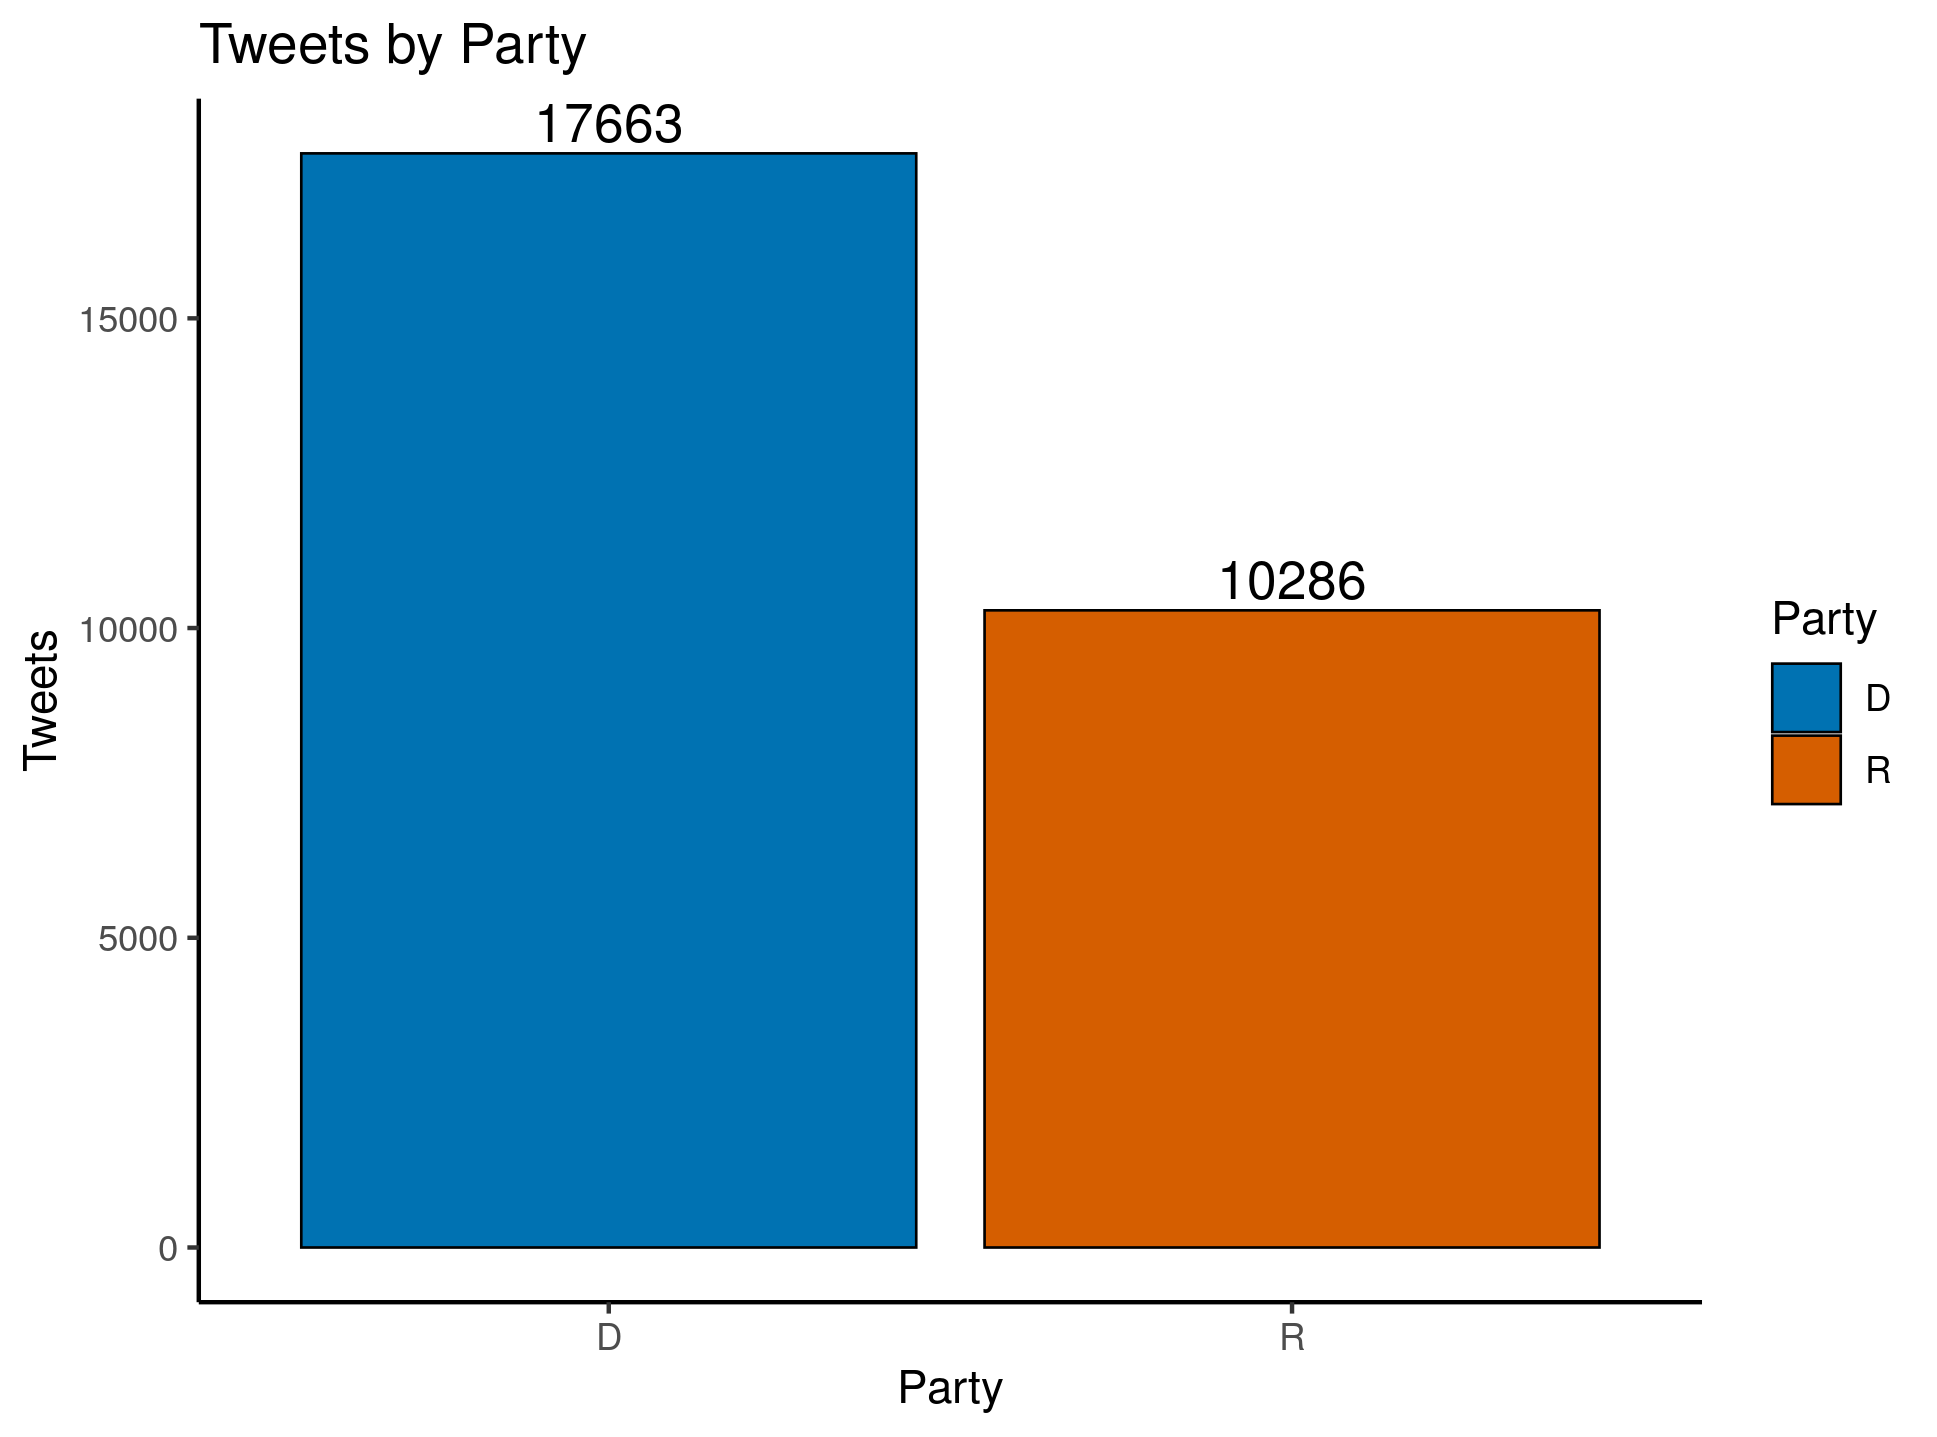
\includegraphics[width=0.66\textwidth]{tweetcount}
\caption{Distribution of tweets}
\label{fig:tweets}
\end{figure}


In conjunction with the text from congress members, I compiled a list of ideologically significant words that represent points of agreement and disagreements between the parties, as well as a list of ideologically neutral words. To generate this list of words, I  first created a list of 100 politically relevant words. I then narrowed this list down to words that have unambiguous meaning, represent clear ideological divides or agreement, and are used more than ten times by each party. For example, “impeach” is a good word for my purposes because of its clear meaning, high usage, and both parties have clear, unified positions.  In addition to the ideologically significant words, I compiled a list of ideologically neutral words that can be found in any context. A word count for each list can be found in table X and a list of these words if found in the appendix.


\begin{table}[h]
 \caption{Key words by category}
  \centering
  \begin{tabular}{lll}
    \toprule
    Category      & \textit{n} & Examples\\
    \midrule
    Disagree      &   29       & trump, abortion, gun\\
    Agree         &   10       & veteran, isis, infrastructure\\
    Base          &   47       & answer, opportunity, member\\
    \bottomrule
  \end{tabular}
  \label{tab:table}
\end{table}

\subsection{Pre-processing and cleaning}
To clean the text I removed websites, emoji, punctuation, and digits via regular expressions. I used spaCy’s language model to tokenize, lemmatize, and remove stop words from the text \cite{honnibal-johnson:2015:EMNLP}. The stop words removed consist of spaCy’s default list with minor alterations to accommodate for specifics in the data set. For example, the word ‘make’ was removed from the list because of its significance to the phrase ‘make America great again.’ A list of stop words is located in the appendix.

Next, I isolate and tag a single word from the aforementioned list of ideologically significant words. This process involves several steps, the first of which is combining synonyms into a single term so that a single word vector can be calculated for a concept. A potential criticism of this process is that by replacing synonyms of words I am compromising some of the semantic meaning of these words. I offer two defenses: First, in all cases the replacement of synonyms into a single term is minor and unambiguous. Examples include replacing President Trump’s twitter handle “@realdonaldtrump” with simply “trump” or replacing the term “leftist” with liberal. Second, differences in terminology primarily reside on ideological fault lines. Because different word vectors are calculated for each ideological group the semantic differences represented by these slight changes in terminology will still largely be represented in the single word vectors and their associated cosine similarity scores. A dictionary of words and their associated synonyms if found in the appendix.

The next step isolates each instance of the key word by inserting spaces between these instances. For example, the string "\#supporttrump" would be altered to "support trump" after the initial cleaning and key word isolation. This allows the word embedding model to treat ‘support’ and "trump" as separate tokens. 

Once key words are isolated, final step is to tag each word with either a political group or randomly assigned label depending on which test I am conduction. If the string "\#supporttrump" was tweeted by a republican, it becomes "support trump\_r." After this process is complete I can calculate a word vector for both trump\_r and trump\_d which represent the Republican and Democratic use of the word ‘trump’ respectively.	

I use Word2vec with a skip-gram architecture as implemented in the python Gensim library to construct embeddings \cite{rehurek_lrec}. Embeddings are trained with word vectors of 100 dimensions and a window size of 10. A complete list of hyper-parameters used to train the model is found in the appendix.

\end{document}